\chapter{Analýza a návrh riešenia}
\label{chap:analyza-navrh-riesenia}
V tejto kapitole je popísaný postup analýzy a návrhu riešenia tejto diplomovej práce. Najprv je popísaná analýza požiadaviek na výslednú aplikáciu a jej primárnu funkcionalitu. Ďalej je popísaný návrh samotnej mobilnej aplikácie, kde sú predstavené prípady užitia a použitia aplikácie, ako aj základný návrh grafického užívateľského rozhrania. Potom nasleduje návrh databáze, ktorý bol realizovaný pomocou ER diagramu. Posledná kapitola pojednáva o návrhu aplikačného rozhrania vychádzajúceho z princípov RESTu.

%%%%%%%%%%%%%%%%%%%%%%%%%%%%%%%%%%%%%%%%%%%%%%%%%%%%%%%%%%%%%%
\section{Analýza požiadaviek}
Analýza požiadaviek čiastočne vychádza z kapitoly 1, v ktorej boli popísané dôležité teoretické znalosti a zároveň vychádza z informácií poskytnutých Fakultnou nemocnicou Brno a jej požiadavok. Podľa týchto informácií a požiadavok by malo ísť o aplikáciu určenú pre platformy Android, iOS a Windows Mobile, ktorá by mala umožňovať vyfotografovať chronickú ranu, primárne preležaninu, spolu s nejakou mierkou. Mierka by mala byť buď pero, alebo prst zdravotnej sestry, prípadne ošetrujúceho lekára a mal by byť nastaviteľný jeho rozmer. Aplikácia by mala byť schopná následne odfotografovanú ranu detekovať, lokalizovať a spočítať plošný rozmer cieľovej plochy, napríklad v milimetroch štvorcových alebo inej miere. V aplikácií by mala byť možnosť prihlásenia užívateľa pomocou sociálnych sietí, ako napríklad Facebook alebo Google+. Ďalej by mal mať užívateľ možnosť svoje snímky pomenovať, porovnať s minulými snímkami, mať možnosť tlače týchto snímok a prípadne ich ukladať na vzdialené úložisko, aby k nim mal prístup aj z iného zariadenia ako je aktuálne používané. Aplikácia by mala byť primárne cielená na zdravotné sestry, poprípade ošetrovateľov starajúcich sa o chronické rany a pomáhať im so sledovaním vývoja rán v čase. 

Z vyššie uvedeného vyplýva, že aplikácia by mala byť dostupná na väčšinu platforiem, aj keď nie v rámci tejto diplomovej práce, ale predovšetkým v rámci dlhšieho časového horizontu vývoja. Z tohoto dôvody bolo usúdené, že by bolo dobré, ak by sa vytvorila hybridná aplikácia, ktorú stačí naprogramovať raz a už iba s drobnými úpravami je ju možné potom publikovať na väčšine dostupných platforiem. Keďže samotné spracovanie obrazu má v hybridných aplikáciách, webových aplikáciách a celkovo v Javasciptovom svete mizivú podporu, tak by spracovanie obrazu (konkrétne detekcia, lokalizácia a určenie plochy) nastávalo vzdialene na servery. Kvôli tomu bolo rozhodnuté, že programová realizácia by mala byť rozdelená na niekoľko logických celkov, ktorých existencia by bola navzájom od seba nezávislá. Mala by sa skladať zo samotnej mobilnej aplikácie, ktorá môže byť chápaná aj ako klientská časť realizácie, keďže ju bude vidieť každý používateľ aplikácie. Ďalej by išlo o databázovú časť, do ktorej by sa ukladali samotné dáta a potrebné informácie spojené s jednotlivými ranami, užívateľmi a snímkami. A nakoniec ako spojovník medzi týmito 2 časťami by figurovalo aplikačné rozhranie vzdialené na serverovej časti, ktoré by komunikovalo s klientskými aplikáciami, ukladalo a získavalo dáta z databáze, umožňovalo autorizáciu a autentifikáciu používateľov, a spracovávalo snímky rán.

%%%%%%%%%%%%%%%%%%%%%%%%%%%%%%%%%%%%%%%%%%%%%%%%%%%%%%%%%%%%%%
\section{Návrh aplikácie}
Návrh samotnej aplikácie bol vypracovaný s rešpektom k analýze požiadaviek. Bolo nutné premyslieť, čoho všetkého by mala byť daná aplikácia schopná, ako by mala plniť svoju úlohu čo najlepšie a čo by mal byť jej hlavný cieľ okrem samotnej detekcie, lokalizácie a určenia plochy chronickej rany. Aplikácia by nemala byť robustným informačným systémom, skôr iba čo možno najjednoduchšie poňatou aplikáciou, zbytočne nezaťažujúcou užívateľa, ale ponúkajúcou dostatočné možnosti pre pomoc so sledovaním chronických rán. Samotný návrh aplikácie bol rozdelený na 2 podkapitoly, a to na návrh funkcionality, alebo toho, čo by mal byť užívateľ schopný vykonávať, a do návrhu užívateľského rozhrania.

\subsection{Návrh funkcionality}
Návrh funkcionality aplikácie bol spracovaný pomocou Diagramu prípadov užitia (Use Case Diagramu), ďalej iba UCD. UCD zobrazuje chovanie systému z pohľadu užívateľa. Jeho účelom je popísať funkcionalitu systému, presnejšie čo presne sa od samotného systému očakáva. Diagram zobrazuje to, čoho má systém, v tomto prípade aplikácia, byť schopný ale už nehovorí o tom, ako sa to bude vykonávať. Diagram je zložený z prípadov užitia (Use Case), aktérov (Actor) a vzťahov medzi nimi. Prípad užitia je sada niekoľkých akcií, ktoré vedú k dosiahnutiu určitého cieľa. Aktér je rola, ktorá komunikuje s jednotlivými prípadmi užitia. UCD je teda v podstate diagram, ktorý zobrazuje všetko to, čo daná užívateľská rola, alebo konkrétny užívateľ môže v systéme vykonávať.

Jedinou rolou v aplikácií, tvorenej v rámci tejto diplomovej práce, je rola všeobecného užívateľa, ktorým je väčšinou zdravotná sestra, lekár, alebo iný ošetrovateľ starajúci sa o chronickú ranu. Každý užívateľ, ktorý si zapne aplikáciou, by sa mal automaticky stať roľou ošetrovateľa. Ošetrovateľ by mal mať možnosť zobraziť si zoznam liečení. Tento zoznam by mal obsahovať liečenia, ktoré aktuálne prebiehajú a sú v určitom štádií, ale zároveň aj liečenia, ktoré už nie sú aktívne pozorované a považujú sa za ukončené. Tento zoznam by mal byť filtrovateľný minimálne podľa stavu liečby a malo by sa v ňom zároveň dať vyhľadávať podľa mena liečeného pacienta. Ďalej by mal byť ošetrovateľ schopný vytvoriť nové liečenie, zobraziť detail už existujúceho liečenia a mať možnosť meniť toto liečenie. Okrem toho by mal mať možnosť zobraziť graf postupu liečenia, konkrétne graf zmeny veľkosti detekovanej plochy chronickej rany a mať možnosť tieto výsledky uložiť do PDF formátu, poprípade vytlačiť. Pre každé liečenie by mal mať možnosť ošetrovateľ potom zobraziť zoznám vytvorených snímkov rán, urobiť novú snímku, zobraziť detail existujúcej snímky, zmeniť snímku a prípadne ju odstrániť. Dôležitým aspektom v aplikácií by mala byť mierka, ktorej význam bude vysvetlený v ďalších kapitolách. Užívateľ aplikácie by mal mať možnosť zobraziť existujúce mierky, tak ako ich aj meniť a odstraňovať. Mierky by sa mali dať tiež pridávať a malo by sa dať voliť, ktorá bude nastavená ako východzia. Celý Diagram prípadov užitia je možné vidieť na obrázku \ref{fig:usecase}.
\begin{figure}[h]
      \centering
      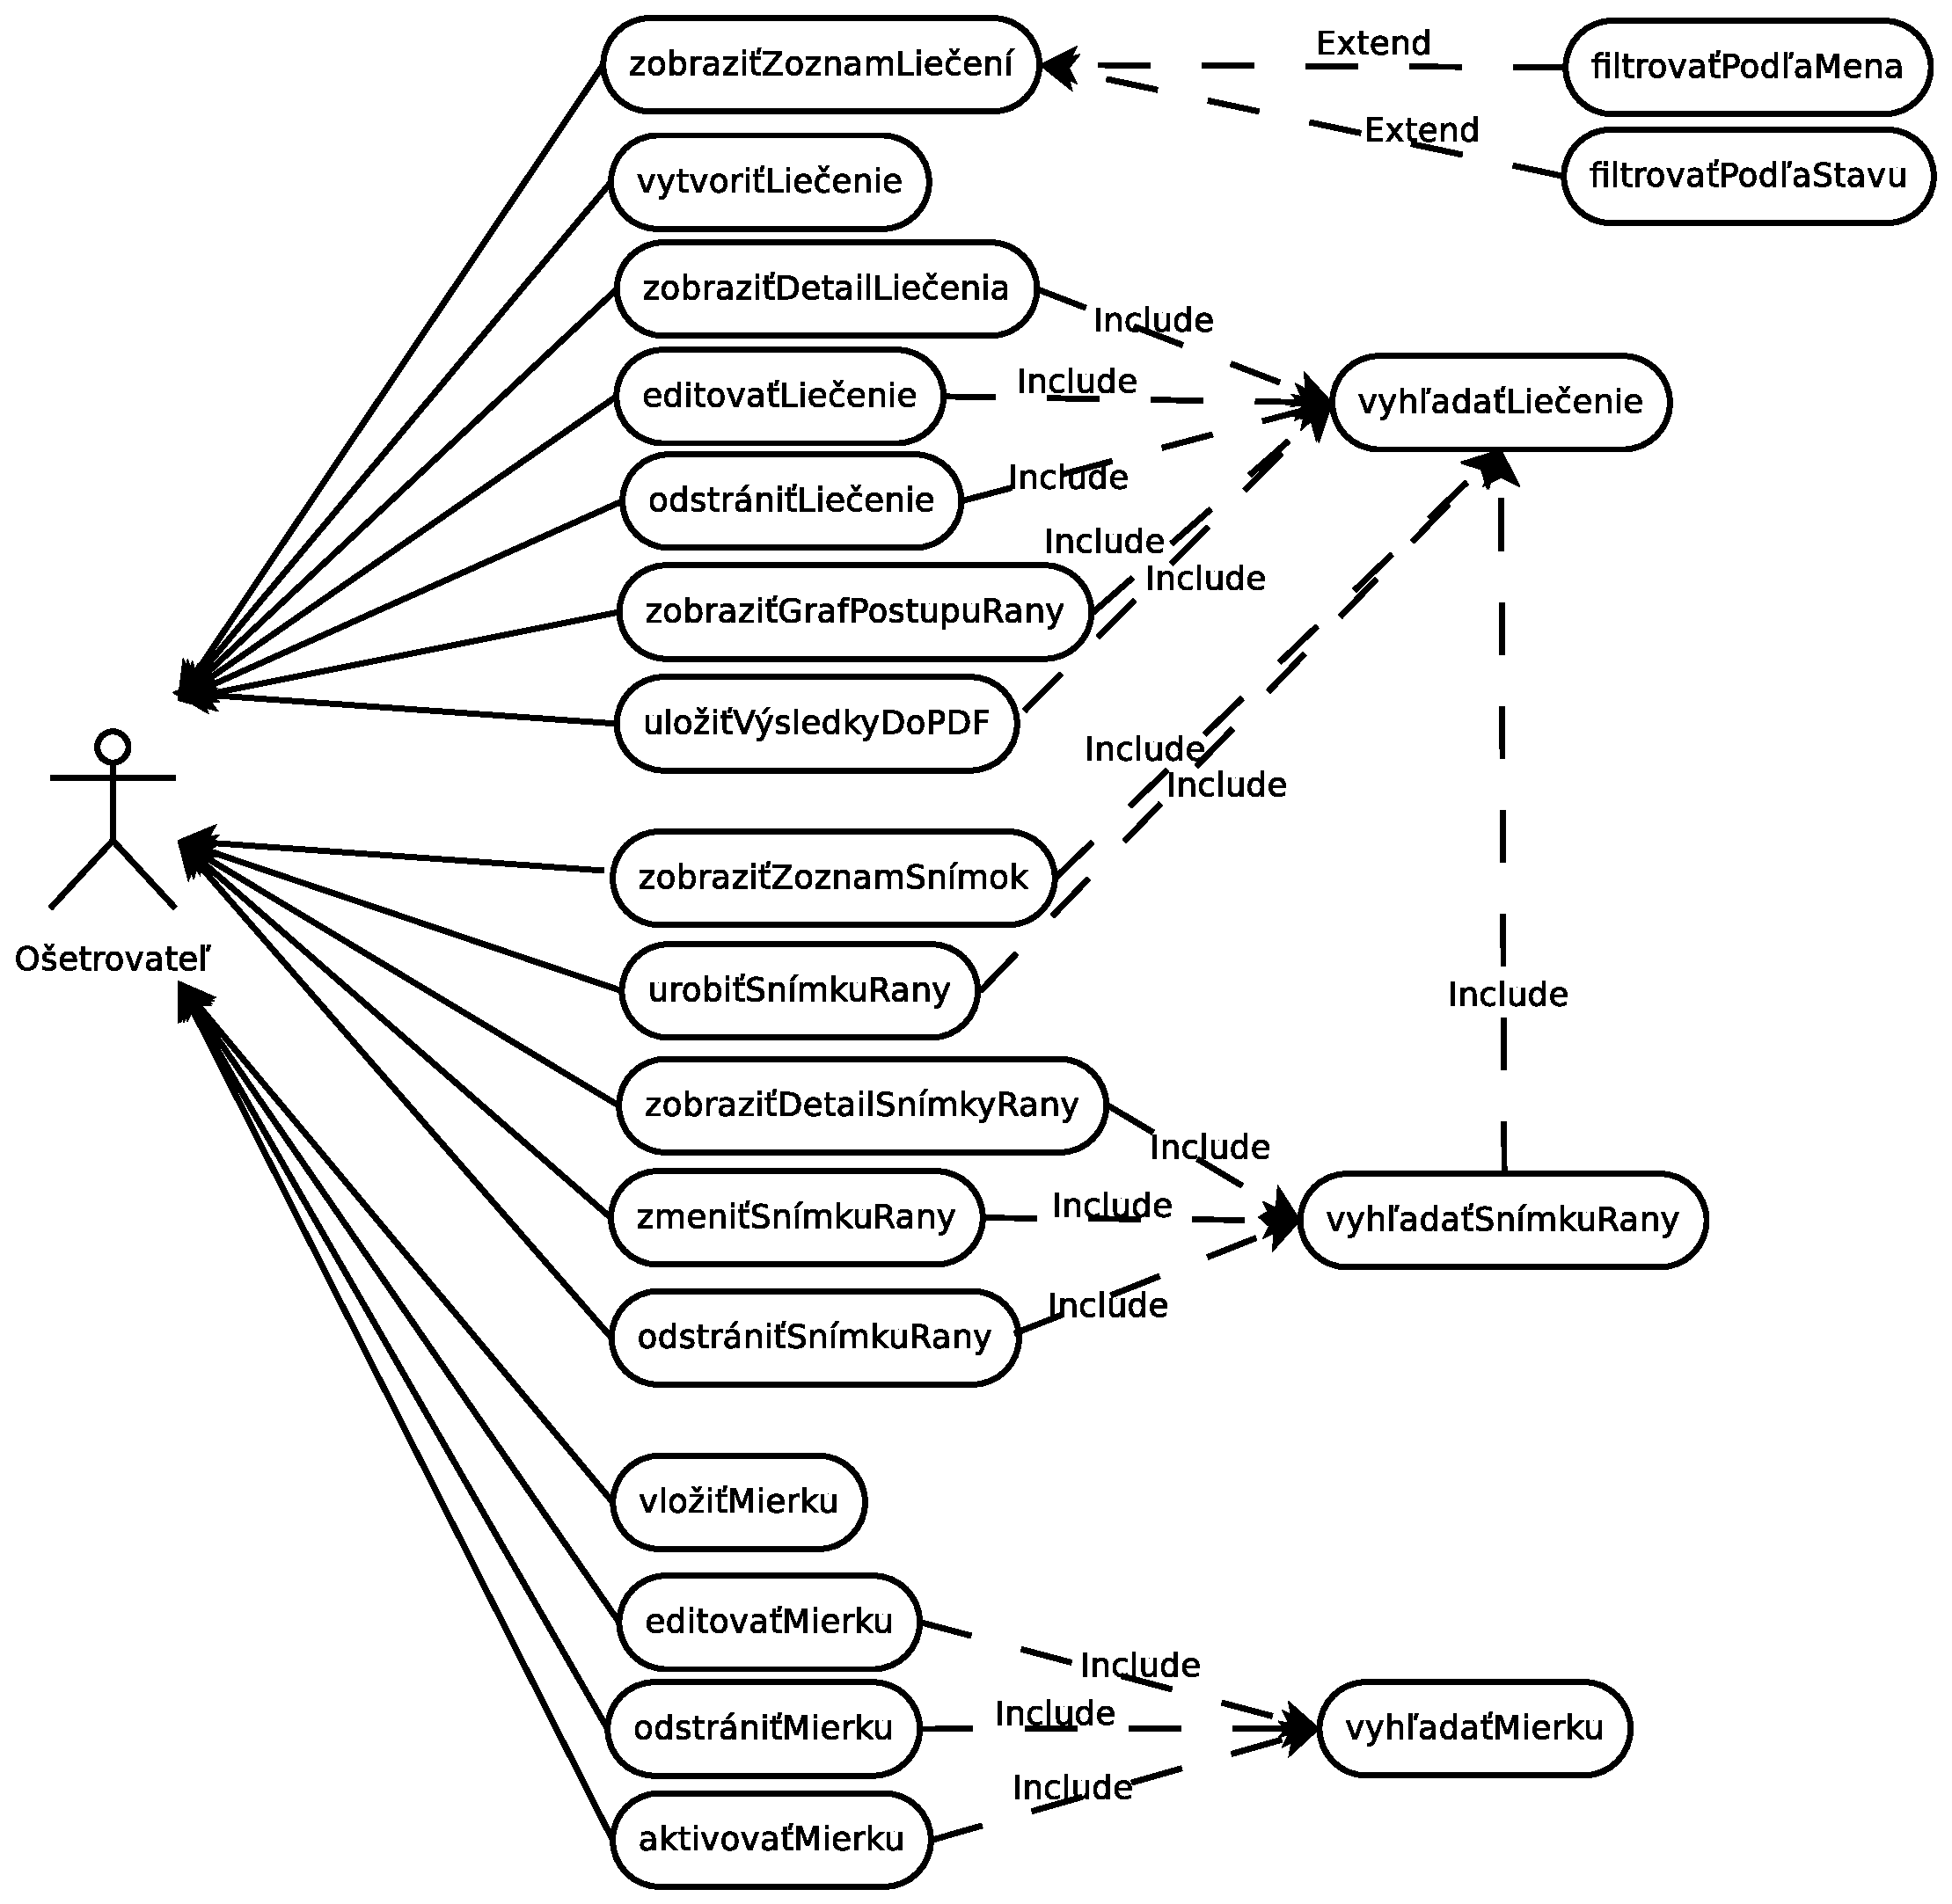
\includegraphics[scale=0.420]{fig/use-case.eps}
      \caption{Diagram prípadov užitia užívateľa aplikácie.}
      \label{fig:usecase}
\end{figure}

\subsection{Návrh grafického užívateľského rozhrania}
Grafické užívateľské rozhranie bolo navrhnuté najprv na papier a potom pre lepšie predstavenie boli tieto náčrty prevedené do digitálnej podoby programom Wireframe Sketcher.

Prvá obrazovka, ktorá bola navrhnutá je obrazovka prihlásenia. Na túto obrazovku by sa mal dostať užívateľ vtedy, keď nie je prihlásený. Typicky sa tak deje pri prvom spustení aplikácie. Pri ďalších spusteniach by si aplikácia mala zapamätať užívateľa a prihlasovať ho už automaticky. Prihlásenie do aplikácie by malo byť povinné a v prípade, že nie je užívateľ prihlásený tak by sa nemalo dať pokračovať ďalej. Na tejto obrazovke by sa malo nachádzať iba tlačidlo na prihlásenie cez nejakú sociálnu sieť, či už Facebook, Google+ alebo obidvoje. Okrem samotného tlačidla by mal byť prítomný aj nejaký vysvetľujúci text. Návrh prihlasovacej obrazovky je možné vidieť na obrázku \ref{fig:mockup1}.
\begin{figure}[h]
      \centering
      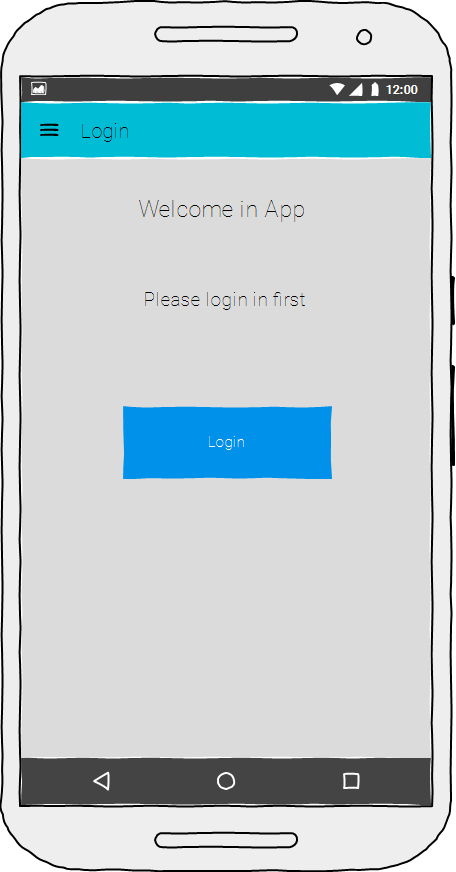
\includegraphics[scale=0.45]{fig/mockup1.png}
      \caption{Obrazovka prihlásenia.}
      \label{fig:mockup1}
\end{figure}

Po prihlásení do systému aplikácie by mal mať užívateľ zobrazený zoznam všetkých liečení, mala by tam existovať možnosť filtrácie a vyhľadávania umiestneného na panely aplikácie a vo vyskakovacom menu. Každý prvok zoznamu by mal mať zobrazené svoje meno liečenia, meno liečeného pacienta a posledný dátum kontroly (lepšie povedané posledný dátum fotografovania rany). V pravom dolnom rohy by malo byť plávajúce tlačidlo na pridávanie liečení. Návrh je možné vidieť na obrázku \ref{fig:mockup4}. 

Po výbere konkrétnej položky by mal byť užívateľ prenesený na obrazovku detailu liečby. V tejto obrazovke by mal mať možnosť vidieť všetky informácie o liečbe (ako napríklad meno pacienta, narodenie pacienta, stav liečby, stav rany...), graf znázorňujúci vývoj rany v čase a zoznam odfotografovaných rán obsahujúci ich mená a dátumy zachytenia snímky. V pravom dolnom rohy by malo byť plávajúce tlačidlo na odfotografovanie rany. Liečbu by bolo možné na tejto obrazovke editovať, poprípade vymazať výberom z vyskakovacieho menu umiestneného v pravom hornom rohu. Mockup je znázornený na obrázku \ref{fig:mockup5}.
\begin{figure}[h]
   \begin{minipage}{0.48\textwidth}
     \centering
     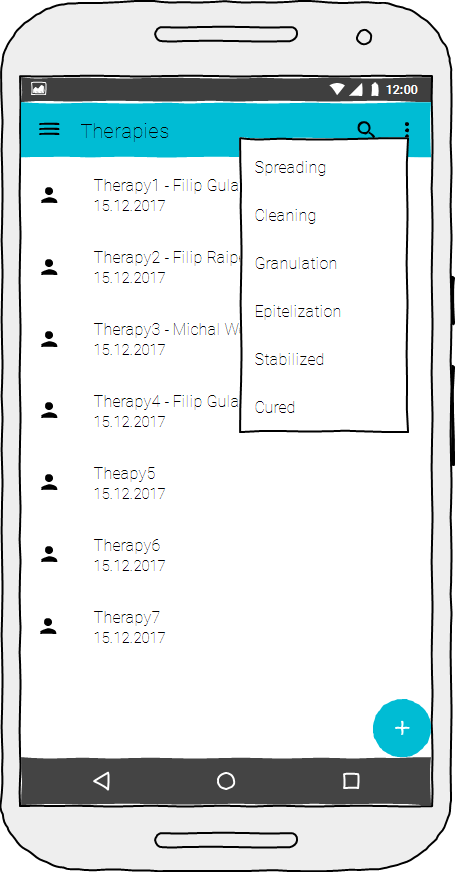
\includegraphics[scale=0.45]{fig/mockup4.png}
      \caption{Obrazovka zoznamu liečení.}
      \label{fig:mockup4}
   \end{minipage}\hfill
   \begin {minipage}{0.48\textwidth}
     \centering
     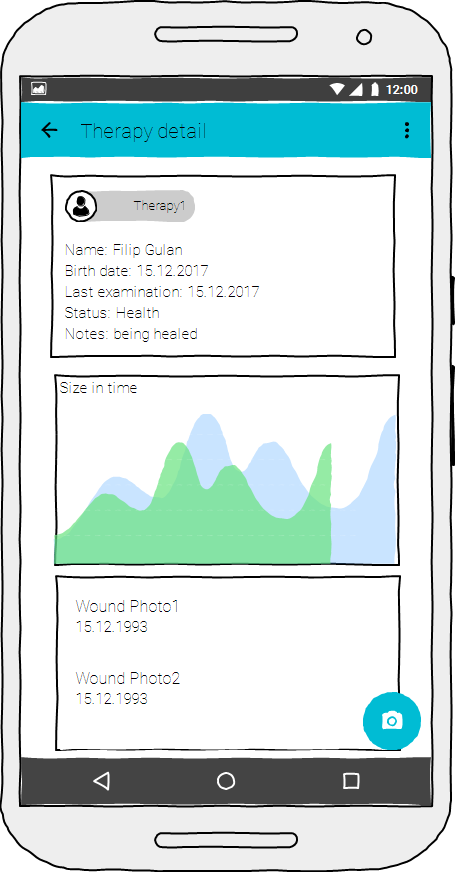
\includegraphics[scale=0.45]{fig/mockup5.png}
      \caption{Obrazovka detailu liečenia.}
      \label{fig:mockup5}
   \end{minipage}
\end{figure}

V prípade, že sa užívateľ rozhodne fotiť ranu, tak by sa mala aktivovať aplikácia kamera, pomocou ktorej by urobil fotku a táto fotografia by bola následne prenesená na server pre detekciu, lokalizáciu a určenie plochy rany. Po tejto detekcií by bola užívateľovi vrátená upravená fotka zo serveru obsahujúca ohraničenie rany a bola by mu zobrazená ako náhľad, podľa ktorého by sa rozhodol, či mu vyhovuje a chce ju zachovať, alebo či chce urobiť vhodnejší snímok rany. Táto obrazovka náhľadu nasnímanej, detekovanej a lokalizovanej rany je možné vidieť na obrázku \ref{fig:mockup6}. 

V prípade, že sa užívateľ rozhodne, že mu odfotografovaný snímok vyhovuje, tak bude prenesený na obrazovku detailu rany. Na tejto obrazovke by sa mali nachádzať základné informácie o aktuálnom snímku rany (ako napríklad meno rany, vypočítaná veľkosť, dátum vykonania snímania a poznámka) a samotná snímka znázorňujúca ranu s jej ohraničením. Na túto obrazovku by sa mal užívateľ dostať aj keď si v detaile liečby vyberie danú konkrétnu fotku rany. Návrh je možné vidieť na obrázku \ref{fig:mockup7}.
\begin{figure}[h]
   \begin{minipage}{0.48\textwidth}
     \centering
     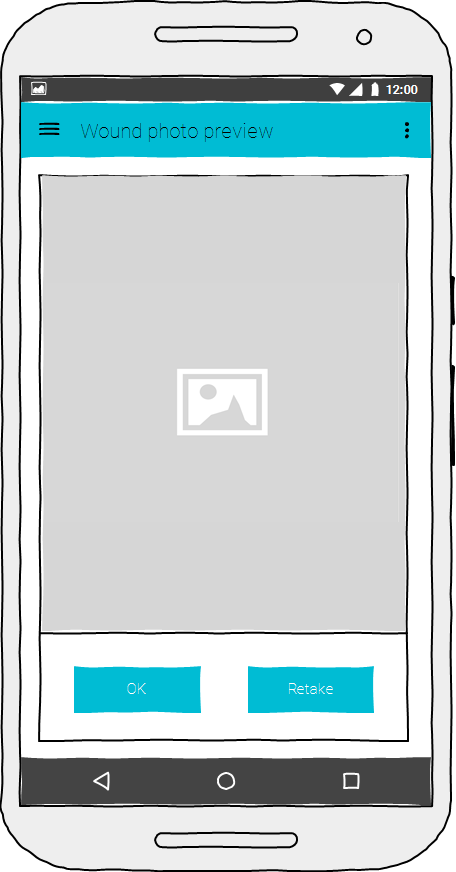
\includegraphics[scale=0.45]{fig/mockup6.png}
      \caption{Obrazovka náhľadu práve získanej a detekovanej rany.}
      \label{fig:mockup6}
   \end{minipage}\hfill
   \begin {minipage}{0.48\textwidth}
     \centering
     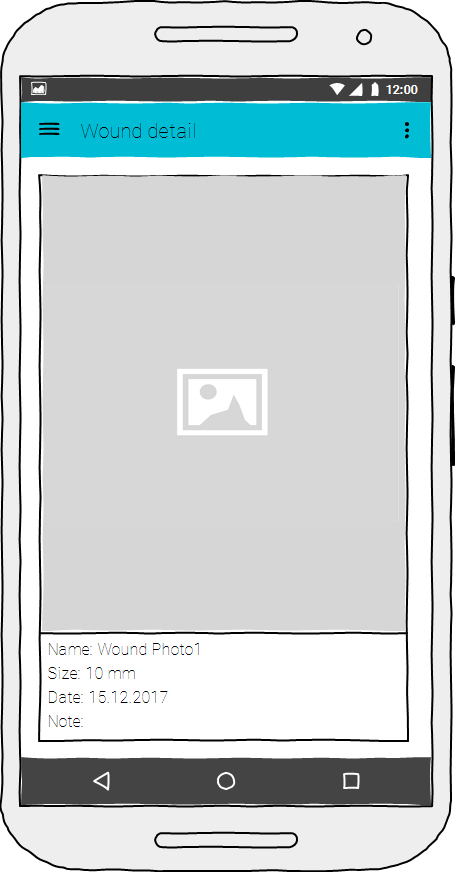
\includegraphics[scale=0.45]{fig/mockup7.png}
      \caption{Obrazovka detailu vyfotenej rany.}
      \label{fig:mockup7}
   \end{minipage}
\end{figure}

Obrázok \ref{fig:mockup2} zobrazuje návrh globálneho menu, ktoré by malo byť dostupné z každej obrazovky. Toto menu by sa malo dať otvoriť z vrchného panelu aplikácie. Malo by obsahovať základné informácie o aktuálne prihlásenom užívateľovi, užívateľ by sa tu mal mať možnosť odhlásiť a mala by tu byť možnosť sa z tohoto menu dostať na obrazovku nastavení.
	
Na obrazovke nastavení zobrazenej na obrázku \ref{fig:mockup3} by sa mali dať spravovať predovšetkým jednotlivé mierky. Mali by sa tu dať pridávať, editovať a vymazávať pomocou kontextového okna. Zároveň by mala byť prítomná možnosť výberu mierky, ktorá sa aplikuje ako východzia.
\begin{figure}[h]
   \begin{minipage}{0.48\textwidth}
     \centering
     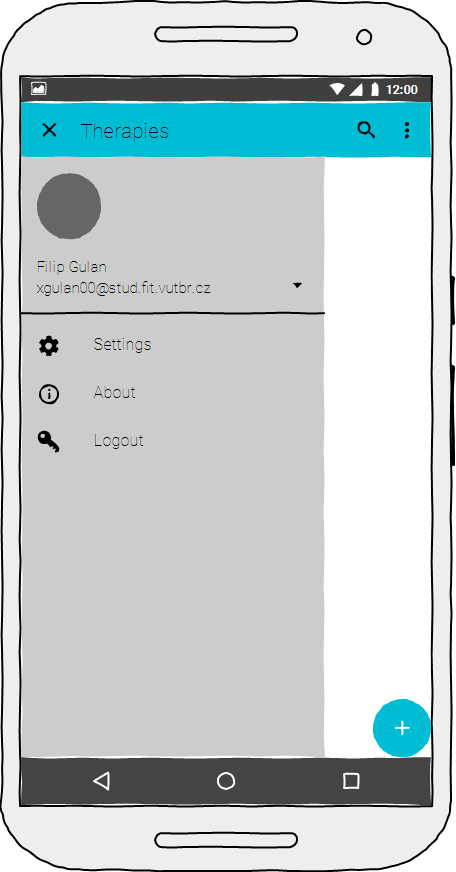
\includegraphics[scale=0.45]{fig/mockup2.png}
      \caption{Globálne menu.}
      \label{fig:mockup2}
   \end{minipage}\hfill
   \begin {minipage}{0.48\textwidth}
     \centering
     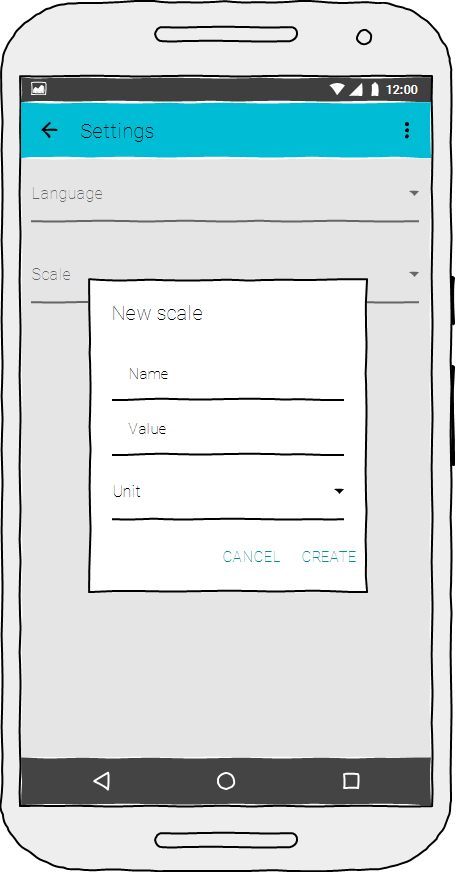
\includegraphics[scale=0.45]{fig/mockup3.png}
      \caption{Obrazovka nastavení a pridávanie mierky.}
      \label{fig:mockup3}
   \end{minipage}
\end{figure}
\newpage

%%%%%%%%%%%%%%%%%%%%%%%%%%%%%%%%%%%%%%%%%%%%%%%%%%%%%%%%%%%%%%
\section{Návrh databáze}
Návrh databáze bol spracovaný pomocou Entity Relationship diagramu, ďalej iba ER diagram, s Unified modeling notáciou. Tento diagram sa používa v softwarovon inžinierstve pre konceptuálne a abstraktné znázornenie dát. Pri modelovaní ER diagramu vzniká jeden z typov konceptuálnych, alebo schematických dátových modelov systému a požiadavok naň z hora dole. V prípade, že sa jedná o návrh informačného systému založeného na databáze a aplikácia tejto diplomovej práce môže byť chápaná ako jednoduchý informačný systém, tak sa tento konceptuálny model v neskoršej fázy mapuje na logický dátový model a ten ďalej na fyzický dátový model.

Návrh využíva informácie  z predchádzajúcej kapitoly o Návrhu aplikácie a samotné návrhy spolu úzko súvisia, keďže funkcionalita pracuje s dátami, ktoré sa získavajú z databáze a zároveň sa do nej ukladajú. Informácie sú tu však podané mierne odlišne, tak aby z nich bolo možné namodelovať ER diagram a uvedomiť si vzťahy medzi jednotlivými entitami. Jednou z hlavných entít figurujúca v tomto databázovom návrhu je liečenie. Liečenie obsahuje svoj názov, aktuálny stav priebehu (ako napríklad dokončené, prebiehajúce, alebo iné). V každom liečení je vždy zapojený jeden konkrétny pacient. A každé liečenie prebieha vždy pod dohľadom jedného konkrétneho ošetrovateľa. Entita pacient obsahuje svoje meno, priezvisko a dátum narodenia. Okrem toho, že pacient podlieha jednému liečeniu, ako už bolo spomenuté, tak každý pacient má jednu ranu, ktorá ho trápi. Táto rana v sebe obsahuje svoj typ, príčinu rany, lokalizáciu a smer rany. Tieto 3 entitné množiny (terapia, pacient a rana) sú modelované ako slabé, z toho dôvodu, že vo výsledku budú brané ako jeden databázový záznam a v diagrame sú oddelené iba pre prehľadnosť návrhu. Nepredpokladá sa, že bude existovať X pacientov s X ranami. Skôr sa predpokladá jeden pacient, na ktorom bude sledovaná jedna rana. A ak by sa náhodou našiel pacient s viac ranami, tak sa iba pridá ďalšie liečenie, čo síce bude znamenať miernu redundanciu dát, ale vo výsledku bude aplikácia jednoduchšia na užívateľské rozhranie, keďže sa nebude musieť vždy vyberať zo zoznamu pacientov, poprípade pridávať nových do tohoto zoznamu. Každá rana môže obsahovať niekoľko svojich snímok a každá snímka patrí práve jednej rane. Každá táto snímka obsahuje svoj názov, veľkosť, dátum snímania, poznámku v prípade potreby. Ďalej snímka obsahuje či je aktuálne rana bolestivá, či zapácha, či sa na nej nachádza sekrét, či obsahuje infekciu a aké sú jej okraje. Každý tento snímok používa vždy jednu konkrétnu mierku a je sledovaná jedným konkrétnym ošetrovateľom. Ošetrovateľ, ktorý môže sledovať niekoľko týchto snímok rán v sebe obsahuje svoje meno, priezvisko, dátum narodenia, svoje heslo k systému a emailovú adresu. Ošetrovateľ môže vlastniť niekoľko mierok, ale minimálne vždy jednu. Poslednou entitou diagramu je mierka. Mierka obsahuje svoje meno, hodnotu a jednotku a vždy patrí práve jednému ošetrovateľovi, ale využívať ju môže niekoľko snímok. Výsledný ER diagram je možné vidieť na obrázku.
\begin{figure}[h]
      \centering
      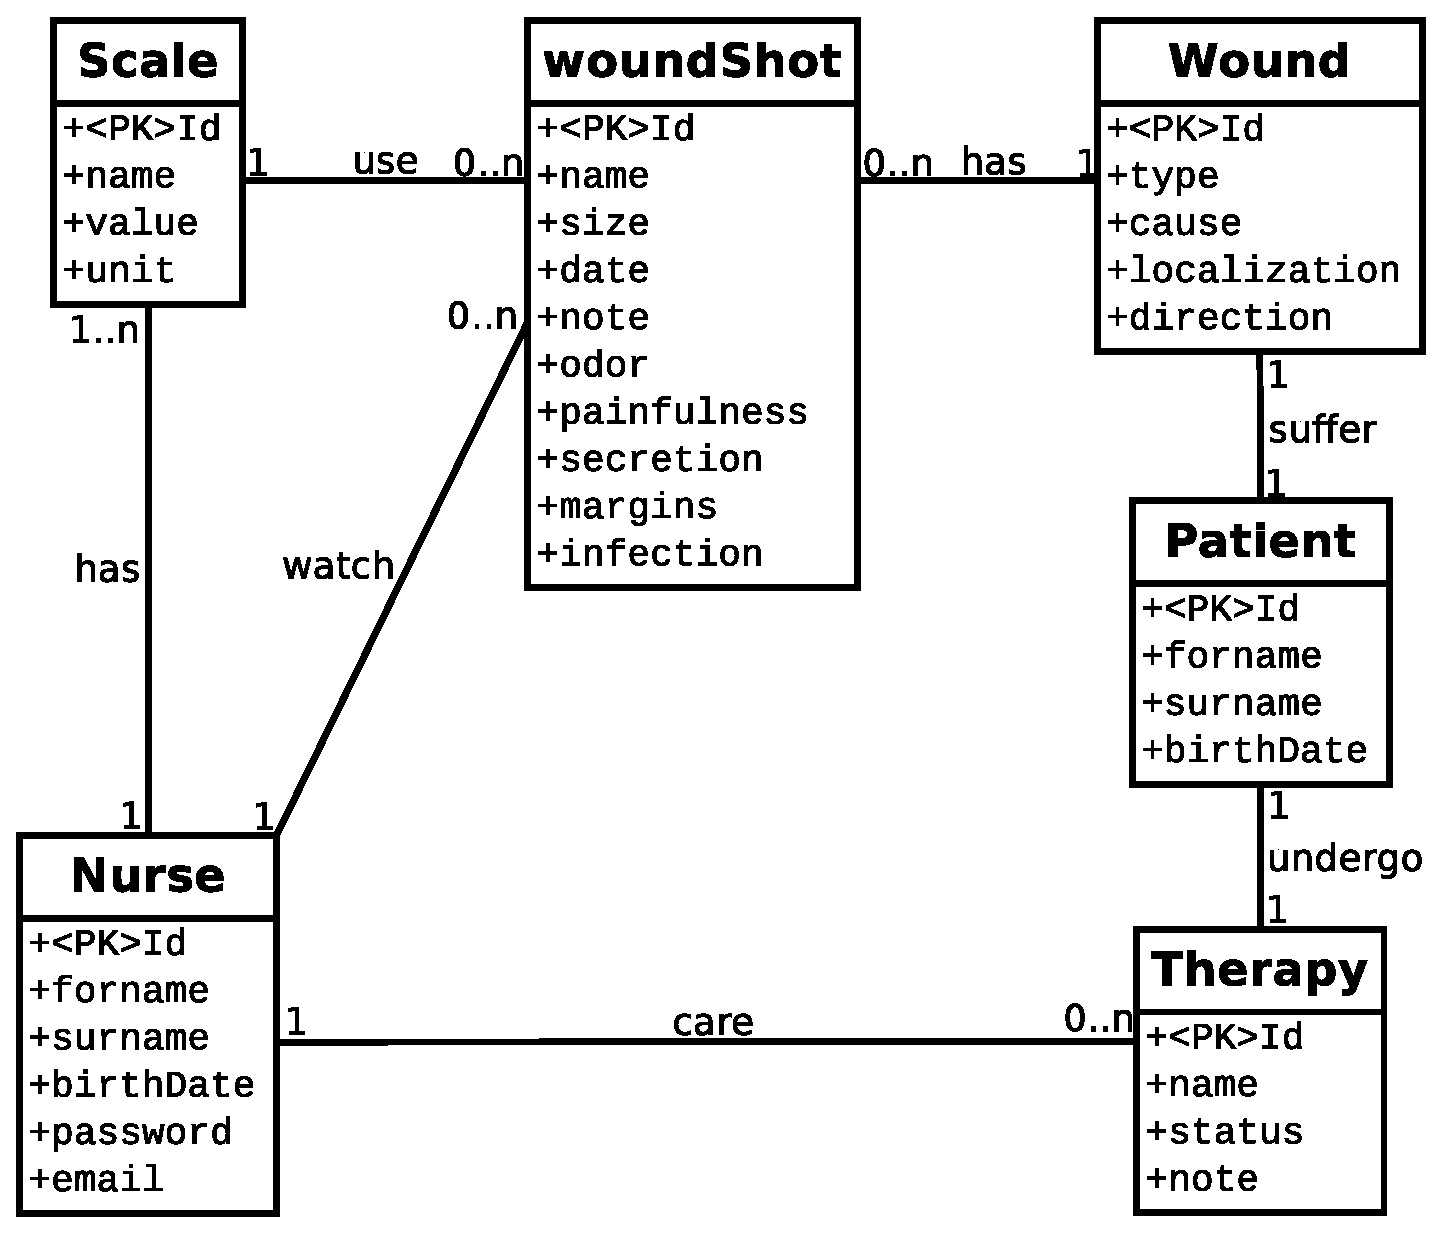
\includegraphics[scale=0.50]{fig/erd.eps}
      \caption{ER diagram návrhu databáze.}
      \label{fig:erd}
\end{figure}

%%%%%%%%%%%%%%%%%%%%%%%%%%%%%%%%%%%%%%%%%%%%%%%%%%%%%%%%%%%%%%
\section{Návrh aplikačného rozhrania}
Aplikačné rozhranie by malo slúžiť ako prostredník medzi samotnou aplikáciou a databázou, ale hlavne tiež by malo slúžiť pre spracovávanie snímok chronických rán, ich detekciu, lokalizáciu a určenie plochy. Celé aplikačné rozhranie nachádzajúce sa na servery by malo byť implementované v duchu REST architektúry. Aplikácia by sa mala dotazovať na server a získavať z neho odpovede. Rozhranie by malo obsahovať 4 základné HTTP metódy ako je GET, POST, PUT a DELETE. Metóda GET by slúžila pre prístup k dátam na uložených na servery, napríklad pre získanie zoznamu liečení, alebo konkrétneho liečenia určeného svojim identifikátorom. Metóda POST by mala slúžiť pre vkladanie dát na server, napríklad pre vytváranie nového liečenia. Metóda PUT by mala slúžiť pre modifikáciu dát na servery, napríklad pre editáciu informácií o liečení. A posledná metóda DELETE by mala slúžiť pre vymazávanie dát zo serveru, napríklad odstránenie liečenia. Príklady všetkých metód na konkrétnom príklade liečení spolu s navrhnutými url adresami, na ktoré by sa malo dať dotazovať je možné vidieť v tabuľke, pričom so všetkými ostatnými dátami by sa malo pracovať rovnako (napríklad pacienti, snímky...).
\begin{table}[h]
\centering
\begin{tabular}{|l|l|l|l|}
\hline
Akcia                      & Metóda & Obsah Body                         & URL         \\ \hline
Získať zoznam liečení      & GET    & NULL                               & /therapy    \\ \hline
Získať liečenie s ID 34    & GET    & NULL                               & /therapy/34 \\ \hline
Vytvoriť nové liečenie     & POST   & \{name: "Name", status: "Active"\} & /therapy    \\ \hline
Editovať liečenie s ID 34  & PUT    & \{name: ''New Name"\}              & /therapy/34  \\ \hline
Odstrániť liečenie s ID 34 & DELETE & NULL                               & /therapy/34  \\ \hline
\end{tabular}
\caption{Príklady pre manipuláciu s liečením prostredníctvom aplikačného rozhrania}
\label{tab:rest-example}
\end{table}

Každý dotaz by mal byť úplne definovaný a mal by obsahovať všetky potrebné informácie k jeho úspešnému vykonaniu. V prípade neúspechu by malo rozhranie vrátiť tomu odpovedajúci špecifický chybový kód. Hlavné a najbežnejšie rozšírené HTTP status kódy je možné vidieť v tabuľke.
\begin{table}[h]
\centering
\begin{tabular}{|l|l|}
\hline
Kód                       & Význam                                                                 \\ \hline
200 OK                    & úspešná operácia a v odpovedi sa nachádzajú dáta  \\ \hline
201 Created               & operácia vkladania dát skončila úspechom                               \\ \hline
204 No Content            & úspešná operácia, ale žiadne dáta sa nenachádzajú v odpovedi \\ \hline
400 Bad Request           & server nerozumie požiadavku, kvôli nesprávnej syntaxi                  \\ \hline
401 Unauthorized          & server pre prístup k dátam vyžaduje autorizáciu                        \\ \hline
403 Forbidden             & server odmietol vykonať požiadavku                                     \\ \hline
404 Not Found             & na servery sa nenašli požadované dáta                                  \\ \hline
500 Internal Server Error & server zaznamenal neočakávanú udalosť                                  \\ \hline
\end{tabular}
\caption{Najbežnejšie používané status kódy HTTP v REST}
\label{tab:rest-codes}
\end{table}